\newpage
\section{Architecture}
The diagram in Figure \ref{fig:Architecture} shows the overview of the components and tasks of all group-members and their interconnections as we proposed. The P2000 notifications are collected and passed through a spelling-check. Next, the notifications are indexed in a database. There is also a database of the codes in the notifications with their associated meaning, which is used to process the notifications. The indexed notifications are then processed to be clustered and possible keywords (to link the notifications to news articles or tweets) are extracted. Based on the location and time of the notifications, news articles and tweets are collected. These are also passed through a spelling-check and are indexed in a database afterwards. The news articles and tweets are then clustered and combined with keywords from the clustered notifications and analyzed to find associations. These associations can then be shown to the user as a single incident that occurred. Also the P2000 notifications, news articles and tweets are classified so the user may search for specific kinds of incidents. \\

The architecture we designed differs a bit from the proposed architecture. The eventual architecture is shown in \autoref{fig:ArchitectureNew}. The first thing changed was that we don't do a spelling check on the notifications anymore. This was not desired because of the codes used in notifications and stemming had no real impact on the performance of indexing notifications. Now on the right-hand side of the architecture we chose to not cluster the news feed and twitter data anymore. The classification of this kind of data proved to be enough to use for the association analyzers. We also had the idea to retrieve keywords from P2000 notifications, but this was hard to do and we did not really need it for the association analyzers. The last changes we made was that the one association analyzer was split into two analyzers. One for notifications and news and one for notifications and twitter messages. At last we also added a GUI to improve the usability of the system.

\begin{center}
\begin{figure}[h!]
  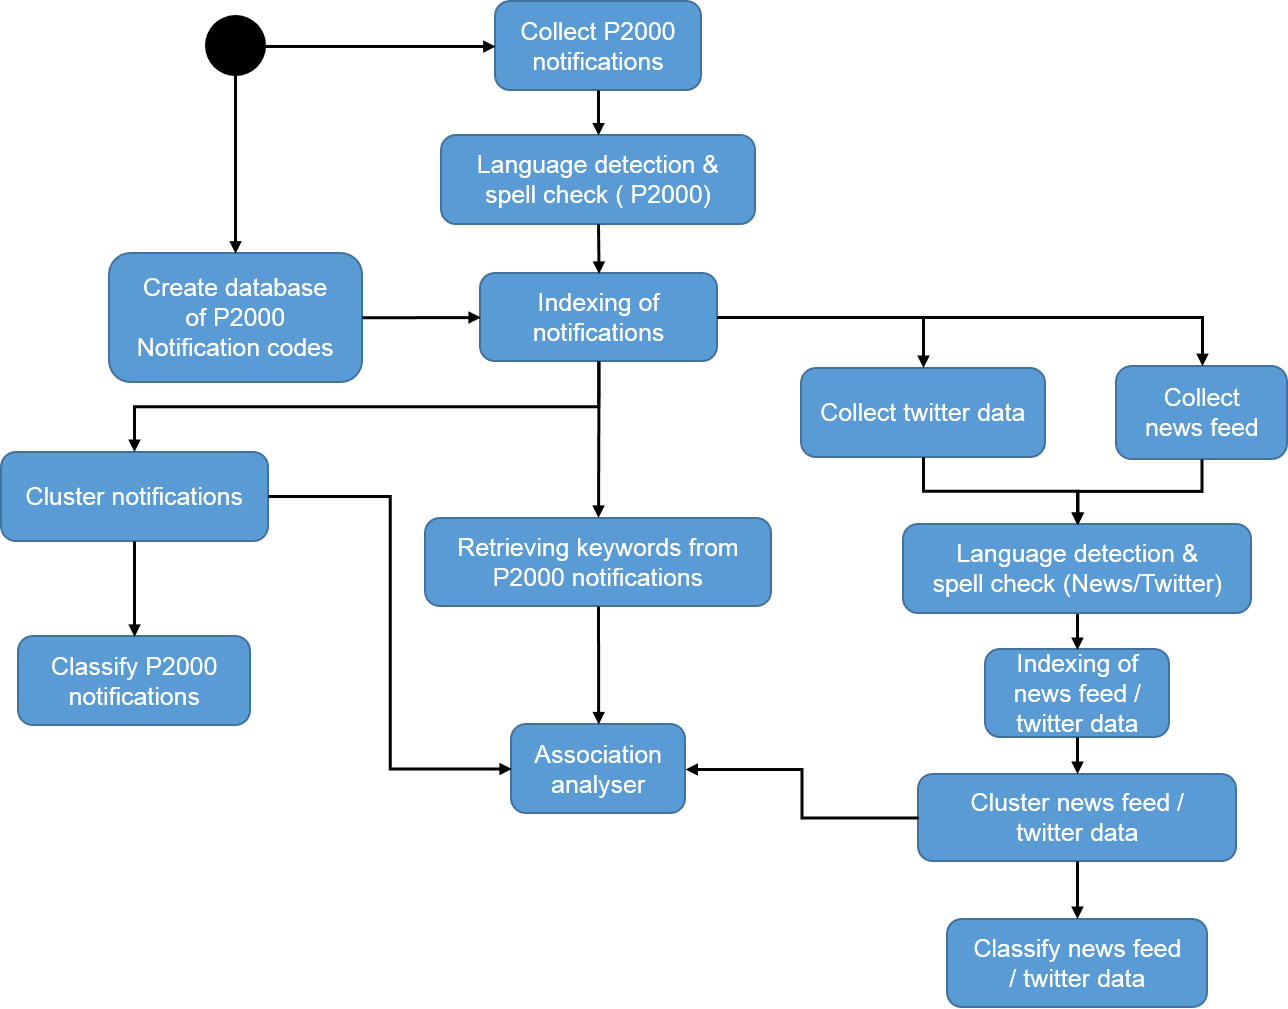
\includegraphics[width=0.85\textwidth]{Architecture.png}
  \caption{Proposed Program architecture}
  \label{fig:Architecture}
\end{figure}

\begin{figure}[h!]
  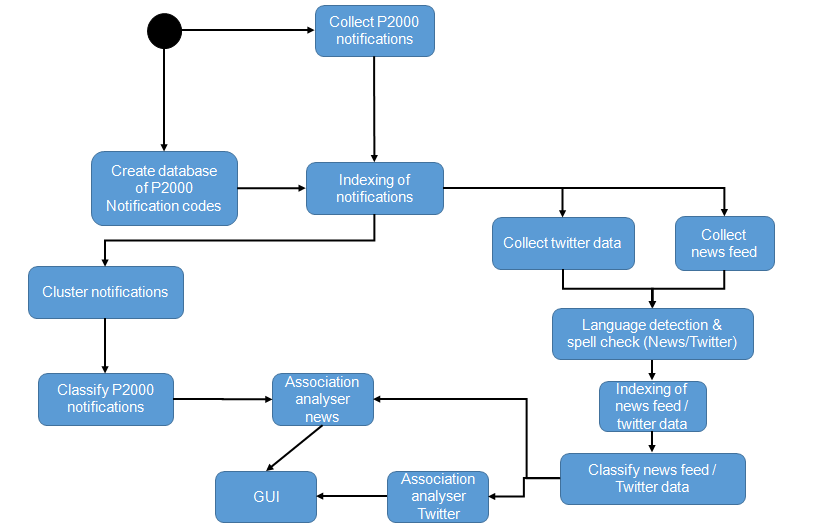
\includegraphics[width=0.85\textwidth]{ArchitectureNew.png}
  \caption{Eventual Program architecture}
  \label{fig:ArchitectureNew}
\end{figure}
\end{center}